\section{Four NP-Complete Problems}
\label{sec:problem-analysis}

In this section we define four PMU placement problems and prove the NP-Completeness of each. We begin with a general overview of NP-Completeness, as well as a high-level description of our proof 
strategy in this paper (Section \ref{subsec:proofstrat}). In the remainder of Section \ref{sec:problem-analysis} we present and prove the NP-Completeness of four PMU placement problems, 
in the following order: \full (Section \ref{subsec:full}), \maxinc (Section \ref{subsec:maxinc}), \xval (Section \ref{subsec:xval}), and \xvalpart (Section \ref{subsec:xvalpart}).

In all four problems defined in this paper, we are only concerned with computing the voltage phasors of each bus (i.e., observing the buses). Using the values of the voltage phasors,
Ohm's Law can be easily applied to compute the current phasors of each transmission line.
Also, we consider networks with both injection and zero-injection buses. For similar proofs for purely zero-injection systems, see our Technical Report \cite{Tech11}.

\subsection{Proof Strategy}
\label{subsec:proofstrat}
Before proving that our PMU placement problems are NP-Complete (abbreviated NPC), we provide some background on NP-Completeness. NPC problems are the hardest problems in complexity class $\mathcal{NP}$. 
It is generally assumed that solving NPC problems is hard, meaning that any algorithm that solves an NPC problem has exponential running time as function of the input size. It is important to clarify that despite being NPC, a {\em specific} problem instance might be efficiently solvable. This is either due to the special structure of the specific instance or because the input size is small, yielding a small exponent. 
For example, in Section \ref{sec:simulations} we are able to solve \full for small IEEE bus topologies due to their small size. Thus, by establishing that our PMU placement problems are NPC, we claim that there {\em exist} bus 
topologies for which these problems are difficult to solve (i.e., no known polynomial-time algorithm exists to solve those cases).  

To prove our problems are NPC, we follow the standard three-step reduction procedure. For a decision problem $\Pi$, we first show $\Pi\in\mathcal{NP}$. Second, we select a known NPC problem, denoted $\Pi'$,
and construct a polynomial-time transformation, $f$, that maps any instance of $\Pi'$  to an instance of $\Pi$. Finally, we ensure that $x\in\Pi'\Leftrightarrow f(x)\in\Pi$ \cite{Garey79}.

Next, we outline the proof strategy we use throughout the paper. In Sections  \ref{subsec:full} through Section \ref{subsec:xvalpart} we modify the approach presented
by Brueni and Heath in \cite{Brueni05} to prove the problems we consider here are NPC. 
In general, we found their scheme to be elegantly extensible for proving many properties of PMU placements.
%For purposes of clarity, we begin by explaining this approach in general terms, and then consider the approach in detail for each problem.

In \cite{Brueni05}, the authors prove NP-Completeness by reduction from planar 3-SAT (\sats). A 3-SAT formula, $\phi$, is a boolean formula in conjunctive normal form (CNF) such that each clause contains at most $3$ literals. For any 3-SAT formula $\phi$ with the sets of variables $\{v_1,v_2, \dots , v_r\}$ and clauses $\{c_1,c_2, \dots , c_s \}$, $G(\phi)$ is the bipartite graph $G(\phi)=(V(\phi),E(\phi))$ defined as follows:
\begin{eqnarray*}
% \nonumber to remove numbering (before each equation)
 V(\phi) &= &\{v_i\; \vert\; 1 \leq i \leq r \} \cup \{c_j \;\vert\; 1 \leq j \leq s \} \\
 E(\phi) &=& \{ (v_i,c_j)\;\vert\; v_i \in c_j\;\; or \;\; \overline{v_i} \in c_j\}.
\end{eqnarray*}
Note that edges pass only between $v_i$ and $c_j$ nodes, and so the graph is bipartite.  \sat is a 3-SAT formula such that $G(\phi)$ is planar \cite{Lich82}. For example, \sat formula
\begin{eqnarray}
	 \varphi &=& (\overline{v_1} \vee v_2 \vee v_3) \wedge (\overline{v_1} \vee \overline{v_4} \vee v_5) \wedge (\overline{v_2} \vee \overline{v_3} \vee \overline{v_5}) \nonumber\\
	 & & \wedge (v_3 \vee \overline{v_4}) \wedge  (\overline{v_3} \vee v_4 \vee \overline{v_5})
\label{eqn:varphi}
\end{eqnarray}
has graph $G(\varphi)$ shown in Figure \ref{fig:gvarphi}. Discovering a satisfying assignment for  \sat is an NPC problem, and so it can be used in a reduction to prove the complexity of the problems we address here. Note that in this work we will use $\varphi$ to denote a specific \sat formula, while $\phi$ will be used to denote a generic \sat formula.

Following the approach in \cite{Brueni05}, for \sat formula, $\phi$, we replace each variable node and each clause node in $G(\phi)$ with a specially constructed set of nodes,
termed a {\em gadget}. In this work, all variable gadgets will have the same structure, and all clause gadgets have the same structure (that is different from the variable gadget structure), and we denote the resulting graph as $H(\phi)$.
In $H(\phi)$, each {\em variable} gadget has a subset of nodes that semantically represent assigning ``True" to that variable, and a subset of nodes that represent assigning it ``False". When a PMU is placed at one of these nodes, this is interpreted as assigning 
a truth value to the \sat variable corresponding with that gadget. 
Thus, we use the PMU placement to determine a consistent truth value for each \sat variable. 
%Reading variable assignments off such a network with PMUs requires that each variable get a consistent truth value via PMU placements.
Also, clause gadgets are connected to variable gadgets at either ``True" or ``False" (but never both) nodes, in such a way that the clause is satisfied if and only if {\em at least one} of those nodes has a PMU.

While we assume $G(\phi)$ is planar, we make no such claim regarding $H(\phi)$, though in practice all graphs used in our proofs are indeed planar. The proof of NPC rests on the fact that solving the underlying $\phi$ formula is NPC.

In what follows, for a given PMU placement problem $\Pi$, we prove $\Pi$ is NPC by showing that a PMU placement in $H(\phi)$, $\Phi$, can be interpreted semantically as describing a satisfying assignment for $\phi$ iff $\Phi\in\Pi$. 
Since \sat is NPC, this proves $\Pi$ is  NPC as well.

While the structure of our proofs is adapted from \cite{Brueni05}, the variable and clause gadgets we use to correspond to the \sat formula are novel, thus leading to a 
different set of proofs. Our work here demonstrates how the work in \cite{Brueni05} can be extended, using new variable and clause gadgets, to address a wide array of PMU placement problems.

%\yyy{Although the structure of our proofs -- form a graph from a \sat formula with variable and clause gadgets -- is adapted from Brueni and Heath  \cite{Brueni05}, 
%they differ significantly in their details. Specifically, Brueni and Heath \cite{Brueni05} assume that all nodes are zero-injection and do not consider cross-validation. As a result,
%the clause and variable gadgets we use in our proofs are distinct from those in \cite{Brueni05}, resulting in significantly different proofs. }


\begin{figure}[t]
\centering
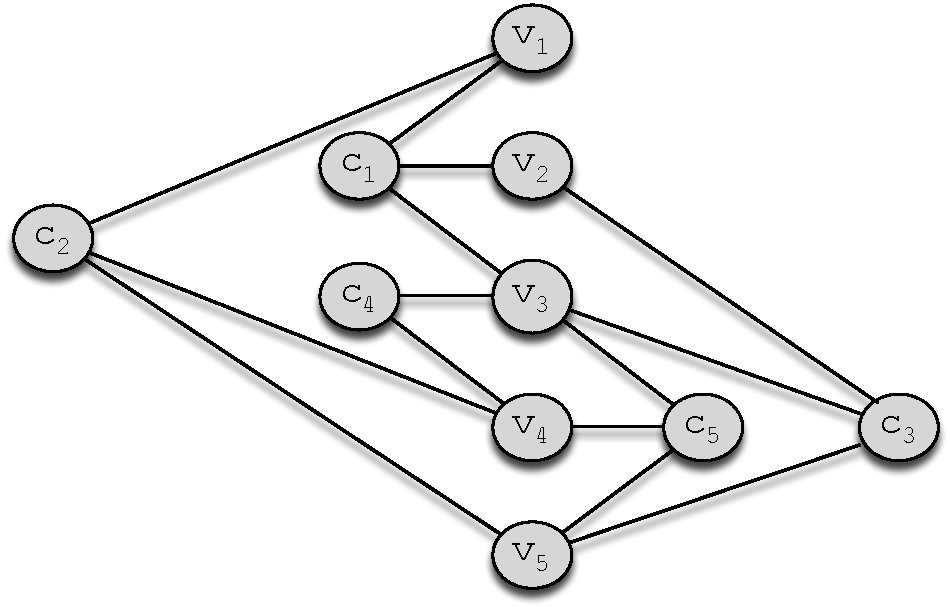
\includegraphics[scale=0.53]{figs/gvarphi.pdf}
\caption{$G(\varphi)=(V(\varphi),E(\varphi))$ formed from $\varphi$ in Equation (\ref{eqn:varphi}). }
\label{fig:gvarphi}
\end{figure}


\subsection{The \full Problem}
\label{subsec:full}

%\begin{figure}[t]
%\centering
%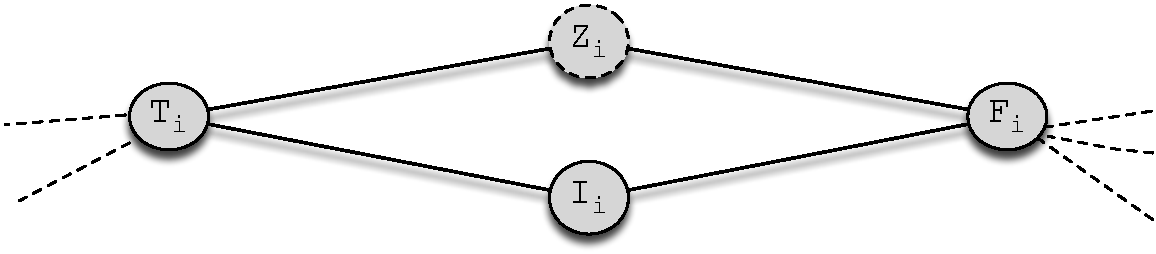
\includegraphics[scale=0.43]{figs/diamond-gadget.pdf}
%\caption{Variable gadget used in Theorem \ref{thm:npc-full}. $Z_i$ is a zero-injection node and all other nodes are injection nodes.}
%\label{fig:diamond-gadget}
%\end{figure}

\begin{figure}[t]
 % \begin{center}
    \fbox{\subfigure[Variable gadget $V_i$ used in Theorem \ref{thm:npc-full} and Theorem \ref{thm:npc-maxinc}.]
    %\fbox{\subfigure[Variable gadget $V_i$ used in Theorem \ref{thm:npc-full} and Theorem \ref{thm:npc-maxinc}. The dashed edges are connections to clause gadgets. $Z_i$ is a zero-injection node and all other nodes are injection nodes.]
	{\label{fig:diamond-gadget}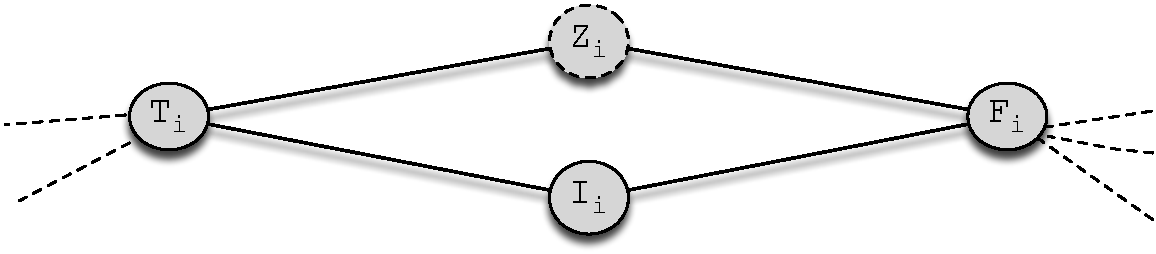
\includegraphics[scale=0.29]{figs/diamond-gadget.pdf}}}
    \fbox{\subfigure[Clause gadget $C_j$ used in Theorem \ref{thm:npc-maxinc}.]
	{\label{fig:line-gadget}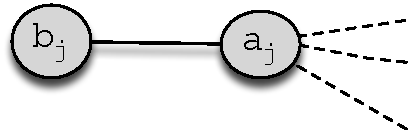
\includegraphics[scale=0.29]{figs/line-gadget.pdf}}}
    %\fbox{\subfigure[Clause gadget $C_j$ used in Theorem \ref{thm:npc-maxinc}. The dashed edges are connections to variable gadgets. $a_j$ and $b_j$ are both injection nodes.]{\label{fig:line-gadget}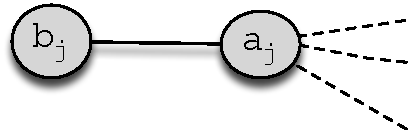
\includegraphics[scale=0.29]{figs/line-gadget.pdf}}}
  %\end{center}
	\caption{Gadgets used in Theorem \ref{thm:npc-full} and Theorem \ref{thm:npc-maxinc}. $Z_i$ in Figure (a) is the only zero-injection node. The dashed edges in Figure (a) are connections to clause gadgets.  Likewise, the dashed edges in Figure (b) are connections to variable gadgets. }
  \label{fig:maxinc}
\end{figure}



The \full problem has been previously discussed in the literature (e.g., the PMUP problem in \cite{Brueni05}, and the PDS problem in \cite{Haynes02}) for purely zero-injection bus systems. Here we consider networks with mixtures of injection and zero-injection buses, and modify the NPC proof for PMUP in \cite{Brueni05} to handle this mixture.

%\full Optimization Problem:
%\begin{itemize}
%	\item \underline{Input}: Graph $G=(V,E)$ where $V=V_Z \cup V_I$ and $V_Z \neq \emptyset$.
%	{\footnote {\small We include the condition that $V_Z \neq \emptyset$ because otherwise \full reduces to \textsc{Vertex-Cover}, making the NP-Completeness
%	proof trivial.}}
%
%	\item \underline{Output}: A placement of PMUs, $\Phi_G$, such that $\Phi^R_G=V$ and $\Phi_G$ is minimal.
%\end{itemize}

\full Decision Problem:
\begin{itemize}
	\item \underline{Instance}: Graph $G=(V,E)$ where $V=V_Z \cup V_I$, $V_Z \neq \emptyset$, $k$ PMUs such that $k \geq 1$.
	{\footnote {\small We include the condition that $V_Z \neq \emptyset$ because otherwise \full reduces to \textsc{Vertex-Cover}, making the NP-Completeness
	proof trivial.}}

	\item \underline{Question}: Is there a $\Phi_G$ such that $|\Phi_G| \leq k$ and $\Phi^R_G = V$?
	%\item \underline{Question}: Is there a $\Phi \subseteq V$ such that $|\Phi| \leq k$ and $m \leq |\Phi^R| < |V|$?
\end{itemize}

The corresponding {\em optimization problem} is to find the minimal value $k$ such that the entire network is observed. It is well-known that these two formulations are equivalent complexity-wise, 
and thus we present and prove only the complexity of the decision problem here. 
%A formal definition of the optimization problem can be found in the Technical Report \cite{Tech12}.
We formally define the optimization problem in our Technical Report \cite{Tech12}.

\begin{theorem}
\full is NP-Complete. %even when restricted to the class of bipartite planar graphs.
\label{thm:npc-full}
\end{theorem}

{\bf Proof Idea}:  We introduce a problem-specific variable gadget. We show that in order to observe all nodes, PMUs must be placed on variable gadgets, specifically on
nodes that semantically correspond to True and False values that satisfy the corresponding \sat formula. 

For our first problem, we use a single node as a clause gadget denoted $a_j$, and the subgraph shown in Figure \ref{fig:diamond-gadget} as the variable gadget. Note that in the variable gadget, all the nodes are injection nodes except for $Z_i$. For this subgraph, we state the following simple lemma:

\begin{lemma}\label{lem:property1}
Consider the gadget shown in Figure \ref{fig:diamond-gadget}, possibly with additional edges connected to $T_i$ and/or $F_i$. Then (a) nodes $I_i, Z_i$ are not observed if there is no PMU on the gadget, and (b) all the nodes in the gadget are observed with a single PMU iff the PMU is placed on either $T_i$ or $F_i$.
\end{lemma}
\begin{proof}
(a) If there is no PMU on the gadget, O1 cannot be applied at any of the nodes, and so we must resort to O2. We assume no edges connected to $I_i,Z_i$ from outside the gadget, and since $T_i,F_i\in V_I$, we cannot apply O2 at them, which concludes our proof.
 
(b) In one direction, if we have a PMU placed at $T_i$, from O1 we can observe $Z_i,I_i$. Since $Z_i$ is zero-injection and one neighbor, $T_i$ has been observed, from O2 at $Z_i$ we can observe $F_i$. The same holds for placing a PMU at $F_i$, due to symmetry.

In the other direction, by placing a PMU at $I_i$ ($Z_i$) we observe $T_i$ and $F_i$ via O1. However, since $F_i,T_i\notin V_Z$, O2 cannot be applied at either of them, so $Z_i$ ($I_i$) will not be observed. \qed
\end{proof}

\begin{proof}[of Theorem \ref{thm:npc-full}]
%\maxinc is easily in $\in \mathcal{NP}$.
We start by arguing that \full $\in \mathcal{NP}$. First, nondeterministically select $k$ nodes in which to place PMUs. Using the rules specified in Section \ref{subsec:observe}, determining
the number of observed nodes can be done in linear time.
%Haynes et al. \cite{Haynes02} show that given a PDS solution can be verified in polynomial time. Since \maxinc only checks $m < |V|$ vertices,
%the same algorithm can be used to verify a \maxinc solution in polynomial time.

To show \full is NP-hard, we reduce from \sats.  Let $\phi$ be an arbitrary \sat formula with variables \\
$\{v_1,v_2, \dots , v_r\}$ and the set of clauses $\{c_1,c_2,\dots , c_s \}$, and $G(\phi)$ the corresponding planar graph. We use $G(\phi)$ to construct a new graph $H_0(\phi) = (V_0(\phi), E_0(\phi))$ by replacing each variable
node in $G(\phi)$ with the variable gadget shown in Figure \ref{fig:diamond-gadget}. The clause nodes consist of a single node (i.e., are the same
as in $G(\phi)$). We denote the node corresponding to $c_j$ as $a_j$. All clause nodes are injection nodes.  In the remainder of this proof we let $H := H_0(\phi)$.
In total, $V_Z$ contains all $Z_i$ nodes for $1 \leq i \leq r$, and all other nodes are in $V_I$.  The edges connecting clause nodes with variable gadgets express which variables are in each clause: for each clause node $a_j$, $(T_i, a_j)\in E_0(\phi) \Leftrightarrow v_i\in c_j$, and $(F_i, a_j)\in E_0(\phi) \Leftrightarrow \overline{v_i}\in c_j$. As a result, the following observation holds:

\begin{observation}\label{obs:1}
For a given truth assignment and a corresponding PMU placement, a clause $c_j$ is satisfied iff $a_j$ is attached to a node in a variable gadget with a PMU. 
\end{observation}


The resulting graph for the example given in Figure \ref{fig:gvarphi} is shown in Figure \ref{fig:proof1-inject-example}.  Nodes with a dashed border are zero-injection nodes. 
{\footnote {\small  Throughout this paper, nodes with dashed borders denote zero-injection nodes. }} 
The corresponding formula for this graph, $\varphi$,
is satisfied by truth assignment $A_{\varphi}$: $\overline{v_1}, \overline{v_2}, v_3, \overline{v_4},$ and $\overline{v_5}$ are True. This corresponds to the dark shaded nodes in Figure
\ref{fig:proof1-inject-example}. While this construction generates a graph with very specific structure, in our Technical Report \cite{Tech12}, we detail how to 
extend our proof to consider graphs with a wider range of structures.% different $\frac{|V_Z|}{|V_I|}$ ratios.


With this construct in place, we move on to our proof. We show that $\phi$ is satisfiable if and only if $k=r=|\Phi_H|$ PMUs
can be placed on $H$ such that $\Phi^R_{H}=V$.

$(\Rightarrow)$ Assume $\phi$ is satisfiable by truth assignment $A_{\phi}$. Then, consider the placement $\Phi_H$ such that for each variable gadget $V_i$, $T_i\in \Phi_H \Leftrightarrow v_i=True$
in $A_\phi$, and  $F_i\in \Phi_H \Leftrightarrow v_i=False$. From Lemma \ref{lem:property1}(b) we know that all nodes in variable gadgets are observed by such a placement. From Observation \ref{obs:1}, all clause nodes are observed because our PMU assignment is based on a satisfying assignment.
Thus, we have shown that $\Phi^R_{H}=V$.

$(\Leftarrow)$
Suppose there is a placement of $r$ PMUs, $\Phi_H$, such that $\Phi_H^R = V$.  From Lemma \ref{lem:property1}(a) we know that for each $V_i$ with no PMU, at least two nodes are not observed, so each $V_i$  must have a PMU placed in it. 
Since we have only $r$ PMUs, that means one PMU per gadget. From Lemma \ref{lem:property1}(b) we know this PMU must be placed on $T_i$ or $F_i$, since otherwise the gadget will not be fully observed. Note that these nodes are all in $V_I$.

Since we assume the graph is fully observed, all $a_j$ are observed by $\Phi_H$. Because we just concluded that PMUs are placed only on injection nodes in the variable gadgets, each clause node $a_j$ can only be observed via application of O1 at $T_i/F_i$ nodes to which it is attached -- specifically, $a_j$ is attached to a node with a PMU. From Observation \ref{obs:1}, all clauses are satisfied by the semantic interpretation of our PMU placement, which concludes our proof. \qed

%Because each clause node, $a_j$, is only connected to $T_i$ or $F_i$ nodes of each variable gadget, $V_i$, and $T_i,F_i \notin V_Z$, each $a_j$ must be observed by applying O1 at an adjacent $T_i$ or $F_i$ node.  Therefore, by assigning
%each $v_i \in \phi$ to $True$ iff $T_i \in \Phi_G$ and each $v_i \in \phi$ to $False$ iff $F_i \in \Phi_G$, we can derive a satisfying truth assignment for $\phi$ from $\Phi_G$. \qed

%Because the $T_i$ and $F_i$ nodes of each variable gadget are connected to clause nodes in exactly the same manner as the $T$ and $F$ variable gadget nodes in \cite{Brueni05},
%we use the proof in \cite{Brueni05} to determine that all clauses in $\phi$ are satisfied by the truth assignment derived from $\Phi_G$. \qed
\end{proof}



\subsection{The \maxinc Problem}
\label{subsec:maxinc}

%Here we define both an optimization and decision version of the \maxinc problem.
\maxinc is a variation of \fulls: rather than consider the minimum number of PMUs required for full system observability,
\maxinc finds the maximum number of nodes that can be observed using a fixed number of PMUs.
To differentiate this problem from \fulls, we assume in the following formulation that we have only $k<k^*$ PMUs at our disposal, i.e., there are not enough PMUs to observe the entire network.

%Before formally stating the \maxinc problem, we present some notation.
%Let $k^*$ be the minimum number of PMUs needed for $\Phi^R = V$. Let $\Phi^R_G$ and $\Phi^R_{G'}$ be the observed nodes for graph $G$ and $G'$, respectively. Finally, $m$ is a
%constant corresponding to a graph $G=(V,E)$ such that $m < |V|$.

%\maxinc Optimization Problem:
%\begin{itemize}
%	\item \underline{Input}: Graph $G=(V,E)$ where $V=V_Z \cup V_I$, $k$ PMUs such that $1 \leq k < k^*$.

%	\item \underline{Output}: A placement of $k$ PMUs, $\Phi_G$, such that $|\Phi^R_G|$ is maximum.
%\end{itemize}

\maxinc Decision Problem:
\begin{itemize}
	\item \underline{Instance}: Graph $G=(V,E)$ where $V=V_Z \cup V_I$, $k$ PMUs such that $1 \leq k < k^*$.

	\item \underline{Question}: For a given $m< |V|$, is there a $\Phi_G$ such that $|\Phi_G| \leq k$ and $m \leq |\Phi^R_G| < |V|$?
\end{itemize}

The corresponding {\em optimization problem} is to find the maximal value $m$ for the given network and $k$ PMUs. A formal definition of the optimization problem can be found in 
our Technical Report \cite{Tech12}. 


\begin{figure}[t]
\centering
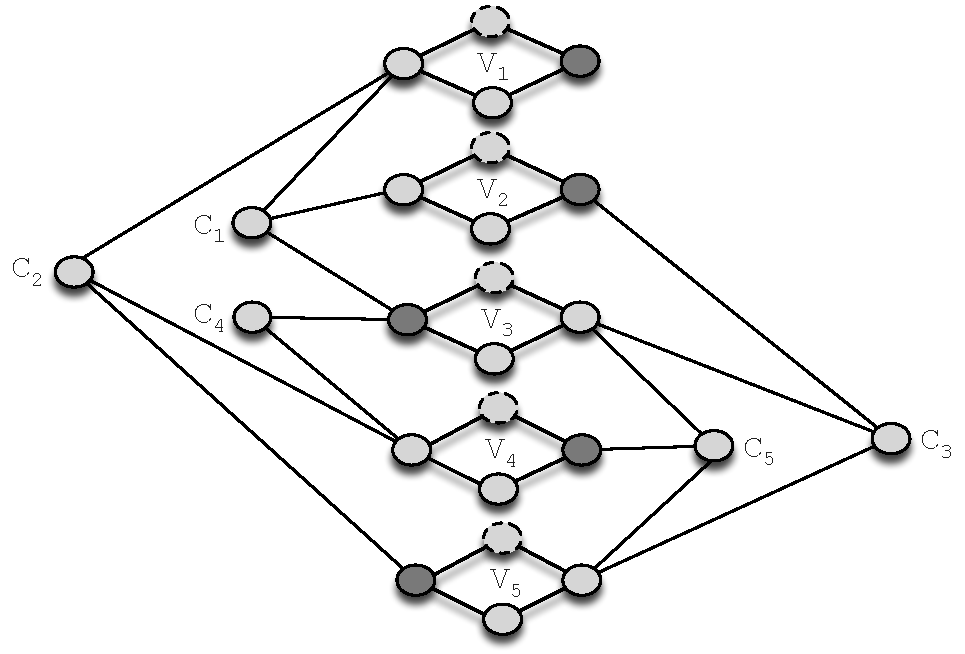
\includegraphics[scale=0.53]{figs/proof1-inject-example.pdf}
%\includegraphics[scale=0.51]{figs/example2.pdf}
\caption{Graph $G=(V,E)=H_1(\varphi)$ formed from $\varphi$ formula in Theorem \ref{thm:npc-full} proof. Nodes with a dashed border are zero-injection nodes.}
\label{fig:proof1-inject-example}
\end{figure}

\begin{theorem}
\maxinc is NP-Complete. %even when restricted to the class of bipartite planar graphs.
\label{thm:npc-maxinc}
\end{theorem}

{\bf Proof Idea}: First, we construct problem-specific gadgets for variables and clauses. We then demonstrate that any solution that observes $m$ nodes must place the PMUs only on nodes
in the variable gadgets. Next we show that as a result of this, the problem of observing $m$ nodes in this graph reduces to Theorem \ref{thm:npc-full}.

\begin{proof}
%\maxinc is easily in $\in \mathcal{NP}$.
\maxinc $\in \mathcal{NP}$ using the same argument in the proof for Theorem \ref{thm:npc-full}.

Next, we reduce from {\sat} as in the proof for Theorem \ref{thm:npc-full}, where $\phi$ is an arbitrary \sat formula. We create a new graph $H_1(\phi) = (V_1(\phi), E_1(\phi))$ which is identical to $H_0(\phi)$ from the previous proof, except that each clause node in $H_0(\phi)$ is replaced with the clause gadget shown in Figure \ref{fig:line-gadget}, comprising of two injection nodes. As before, the edges connecting clause nodes with variable gadgets express which variables are in each clause: for each clause node $a_j$, $(T_i, a_j)\in E_1(\phi) \Leftrightarrow v_i\in c_j$, and $(F_i, a_j)\in E_1(\phi) \Leftrightarrow \overline{v_i}\in c_j$. Note that Observation \ref{obs:1} holds here as well.



% Before beginning our proof that \maxinc is NP-hard, we briefly summarize the reduction from \sat used in \cite{Brueni05}.
% Given a \sat formula, $\phi$, with variables $\{v_1,v_2, \dots , v_r\}$ and the set of
% clauses $\{c_1,c_2, \dots , c_s \}$, a graph $H(\phi) = (V(\phi),E(\phi))$ is formed as follows.  Each variable, $v_i$, is replaced with a gadget shown in Figure \ref{fig:variable-gadget}.  Each
% clause, $c_j$, is replaced with a 2-clique $C[j],C'[j]$.  The edges in $E(\phi)$ represent whether a clause contains a variable.  If the variable $v_i$ occurs in clause $c_j$, $C[j]$ is connected to
% $v_i$'s $T$ node. Conversely, if $\overline{v_i}$ occurs in clause $c_j$, then $C[j]$ is connected to $v_i$'s $F$ node.
% Figure \ref{fig:proof1-example} shows the graph $H(\varphi)$ formed from \sat formula $\varphi$, defined in Equation (\ref{eqn:varphi}), with one exception:
% for each clause gadget, $C_j$, $C_j$'s two leaf nodes are removed.

% In our proof, we define the same \sat formula, $\phi$, as in \cite{Brueni05}: $\phi$ has variables $\{v_1,v_2, \dots , v_r\}$ and the set of clauses $\{c_1,c_2, \dots , c_s \}$.
% From $\phi$, we create a graph $G=(V,E)$ which is identical to $H(\phi)$ defined in \cite{Brueni05} with one exception. We replace each 2-clique $\{C[j],C'[j]\} \in H(\phi)$ with
% clause gadget $C_j$. Each $C_j$ has the following $\Gamma$ functions: $\Gamma(d_j) = \{b_j\}$, $\Gamma(e_j) = \{b_j\}$, $\Gamma(b_j) = \{a_j,d_j,e_j\}$, and $\Gamma(a_j) = \Gamma_o(C[j]) \cup \{b_j\}$
% where $\Gamma_o(C[j])$ is the $\Gamma$ function for $C[j] \in H(\phi)$. $C_j$ is shown in Figure \ref{fig:clause-gadget}.

% For example, the graph for formula $\varphi$ defined in Equation (\ref{eqn:varphi}) is shown in Figure \ref{fig:proof1-example}.
% $\varphi$ is satisfied by truth assignment $A_{\varphi}$: $\overline{v_1}, \overline{v_2}, v_3, \overline{v_4},$ and $\overline{v_5}$ are true.
% The dark shaded nodes have PMUs and correspond to $A_{\varphi}$.

We are now ready to show \maxinc is NP-hard. For convenience, let $H := H_1(\phi)$.  Recall $\phi$ has $r$ variables and $s$ clauses. 
Here we consider the instance of \maxinc where $k=r$ and $m = 4r + s$, and show that $\phi$ is satisfiable if and only if $r=|\Phi_H|$ PMUs
can be placed on $H$ such that $m \leq |\Phi^R_{H}| < |V|$. In our Technical Report \cite{Tech12}, 
we extend this proof to allow arbitrary $m$ values and different $\frac{|V_Z|}{|V_I|}$ ratios.
%we discuss how to extend this proof for any larger value of $m$ and different$\frac{|V_Z|}{|V_I|}$ ratios.

$(\Rightarrow)$ Assume $\phi$ is satisfiable by truth assignment $A_{\phi}$. Then, consider the placement $\Phi_H$ such that for each variable gadget $V_i$, $T_i\in \Phi_H \Leftrightarrow v_i=True$
in $A_\phi$, and  $F_i\in \Phi_H \Leftrightarrow v_i=False$.  In the proof for Theorem \ref{thm:npc-full} we demonstrated such a placement will observe all nodes in $H_0(\phi)\subset H_1(\phi)$, and using the same argument it can easily be checked that these nodes are still observed in $H_1(\phi)$. Each $b_j$ node remains unobserved because each $a_j \in V_I$ and consequently O2 cannot be applied at $a_j$.
Since $|H_0(\phi)|=4r+s = m$, we have observed the required nodes.

$(\Leftarrow)$
We begin by proving that any solution that observes $m$ nodes must place the PMUs only on nodes in the variable gadgets. By construction, each PMU is either on a clause gadget or a variable gadget, but not both. Let $0\leq t\leq r$ be the number of PMUs on clause gadgets, we wish to show that for the given placement $t=0$. First, note that {\em at least} $\max(s-t,0)$ clause gadgets are without PMUs, and that for each such clause (by construction) at least one node ($b_i$) is not observed. Next, from Lemma \ref{lem:property1}(a) we know that for each variable gadget without a PMU, at least two nodes are not observed.

Denote the {\em unobserved} nodes for a given PMU placement as $\Phi_H^-$. Thus, we get $|\Phi_H^-| \geq 2t + \max((s-t), 0)$. However, since $m$ nodes are observed and  $|V|-m \leq s$, we get $|\Phi_H^-| \leq s$, so we know $s \geq 2t + \max((s-t), 0)$. We consider two cases:
\begin{itemize}
	\item $s\geq t$: then we get $s \geq t + s \Rightarrow t=0.$
	\item $s < t$:	then we get $s \geq 2t$, and since we assume here $0\leq s < t$ this leads to a contradiction and so this case cannot occur.
\end{itemize}

Thus, the $r$ PMUs must be on nodes in variable gadgets. Note that the variable gadgets in $H_1(\phi)$ have the same structure as in $H_0(\phi)$. We return to this point shortly.

Earlier we noted that for each clause gadget without a PMU, the corresponding $b_j$ node is unobserved, which comes to $s$ nodes. To observe $m=4r+s$ nodes, we will need to observe all the remaining nodes. Thus, we have reduced the problem to that of observing all of $H_0(\phi)\subset H_1(\phi)$. Our proof for Theorem \ref{thm:npc-full} demonstrated this can only be done by placing PMUs at nodes corresponding to a satisfying assignment of $\phi$, and so our proof is complete. \qed
\end{proof}
%Finally, we show that $G$ is bipartite and planar. From \cite{Brueni05} we know that $H(\phi)$ is bipartite and planar.  Recall, the only difference between $G$ and $H(\phi)$ is that $G$'s clause
%gadgets have two extra nodes: $d_j$ and $e_j$.  We must show that the addition of all $d_j$ and $e_j$ to $H(\phi)$ maintains the condition that the resulting graph, $G$, is bipartite and planar.
%We add $d_j$ and $e_j$ to the same partition as $a_j$, $V_1$.
%Because $d_j$ and $e_j$ are only connected to $b_j$ and $b_j \notin V_1$,
%this maintains the condition that $G$ is bipartite.

%By definition every \sat formula, $\phi$, has a planar embedding $G(\phi)$.  From \cite{Brueni05} we know that $H(\phi)$ maintains the planar
%embedding. By inspection, adding $d_j$ and $e_j$ to $H(\phi)$ preserves the condition that $G$ is planar.
%\end{proof}


\subsection{The \xval Problem}
\label{subsec:xval}

%First we dedine \xval as an optimization problem and then state then state the \xval as a decision problem.

%\xval Optimization Problem:
%\begin{itemize}
%	\item \underline{Input}: Graph $G=(V,E)$ where $V=V_Z \cup V_I$.
%
%	\item \underline{Output}: A placement of PMUs, $\Phi_G$, such that $\Phi^R_G = V$,
%	and  $\Phi_G$ is minimal under the condition that each $v \in \Phi_G$ is cross-validated according to the rules specified in Section \ref{subsec:xval}.
%\end{itemize}

\xval Decision Problem:
\begin{itemize}
	\item \underline{Instance}: Graph $G=(V,E)$ where $V=V_Z \cup V_I$, $k$ PMUs such that $k \geq 1$.

	\item \underline{Question}: Is there a $\Phi_G$ such that $|\Phi_G| \leq k$ and $\Phi^R_G = V$ under the condition that each $v \in \Phi_G$ is cross-validated?
	%\item \underline{Question}: Is there a $\Phi_G$ such that $|\Phi_G| \leq k$, $\Phi^R_G = V$, and each $v \in \Phi_G$ is cross-validated?
	%\item \underline{Question}: Is there a $\Phi \subseteq V$ such that $|\Phi| \leq k$, $\Phi^R = V$, and each $\phi \in \Phi$ is cross-validated?
\end{itemize}

The corresponding {\em optimization problem} is to find the minimal $k$ such that the entire network is observed and all PMUs are cross-validated. 
%A formal definition of the optimization problem can be found in our Technical Report \cite{Tech12}. 
The optimization problem is formally defined in our Technical Report \cite{Tech12}.

\begin{figure}[t]
\centering
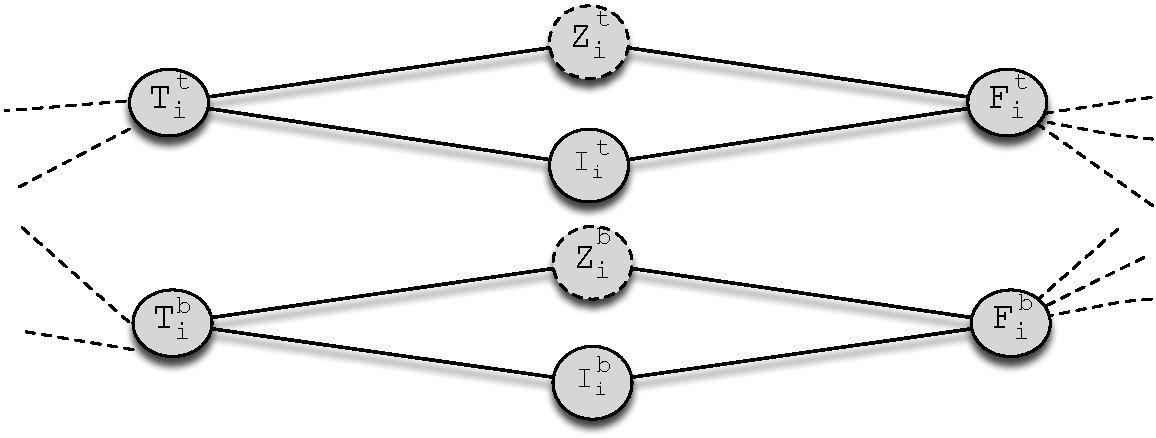
\includegraphics[scale=0.46]{figs/vgadget-inject.pdf}
%\includegraphics[scale=0.51]{figs/example2.pdf}
\caption{Variable gadget used in Theorem \ref{thm:npc-xval}, containing two disconnected subgraphs. Superscript, $t$, denotes nodes in the upper subgraph and 
superscript, $b$, indexes nodes in the lower subgraph. The dashed edges are connections to clause gadgets.}
%\caption{Variable gadget used in Theorem \ref{thm:npc-xval} proof.  The gadget has two disconnected subgraphs, where the superscript, $t$, denotes nodes in the upper subgraph and 
%superscript, $b$, indexes nodes in the lower subgraph. The dashed edges are connections to clause gadgets.}
\label{fig:xval-gadget}
\end{figure}

\begin{theorem}
\xval is NP-Complete. % even when restricted to the class of bipartite and chordal graphs.
\label{thm:npc-xval}
\end{theorem}

% {\bf Proof idea:} We show \xval is NP-hard by reducing from \sats.  Similar to our redcution
% for \maxincs, we create a clause gadget for each clause in \sat forumula, $\phi$, and a variable gadget
% for each variable in $\phi$.  The clause gadget is a pair of nodes connected by an edge.  The variable
% gadget is shown in Figure \ref{fig:xval-gadget}.  A variable gadget, $V_i$, is connected to the clause gadgets, $C_j$, only if
% variable $v_i$ appears in clause $c_i$ in $\phi$.
%
% %If a variable, $v_i$, appears in clause, $c_j$,
% %$c_j$'s clause gadget has the edges $(C[j], T_t), (C[j],T_b)$. Similarily, if clause $c_j$
% %contains variable $\overline{v_i}$ in $\phi$, the $c_j$'s clause gadget has the edges $(C[j], F_t), (C[j],
% %F_b)$.
%
% We place PMUs on variable gadget nodes $T$ and $F$ according to the literal value of each variable in the satisfying truth assignment for $\phi$.
% %PMUs at $T$ nodes are cross-validated using XV2 via the common clause node.
% This leads to a fully observed graph in which all PMUs are cross-validated.  In the other direction, we show that $G$ can only be fully observed
% if $2$ PMUs are placed on each variable gadget. Specifcally, PMUs must be placed on both $T$ nodes or both $F$ nodes, in each variable gadget.  We use the PMU placement
% to derive a satisfying truth assignment for \sat formula $\phi$.
%All clause nodes are observed because each clause is adjacent to at least one PMU node.  The variable clauses are
%Given a satisfying truth assingment to $\phi$, we place PMUs $T$ nodes and $F$ nodes only.
%If a variable $v_i \in \phi$ is True, we place a PMU on each of the $T$ nodes of $v_i$ corresponding variable gadget.  Likewise,
%if $v_i$ is false, a PMU is placed on the $F$ nodes of $v_i$'s variable gadget.

% variable gadgets and clause gadgets
% => place PMUs on T/F nodes of each variable gadget
% <= in order for G to be fully observed each variable gadget must have 2 PMUs,  in order to satisfy cross-validation
%   must be on T/F nodes.  PMU on T node implies variable is true and vice versa.  in this way we derive a satisfying assignment for $\phi$
%

{\bf Proof Idea:}   We show \xval is NP-hard by reducing from \sats.  
We create a single-node gadget for clauses (as for \fulls) and the gadget shown in Figure \ref{fig:xval-gadget} for each variable. Each variable gadget here comprises of two disconnected components, 
and there are two $T_i$ and two $F_i$ nodes, one in each component. First, we show that each variable gadget must have $2$ PMUs for the entire graph to be observed, one PMU for each subgraph.
Then, we show that cross-validation constraints force PMUs to be placed on both $T$ nodes or both $F$ nodes.  Finally, we use the PMU placement to derive a satisfying \sat truth assignment.
 
%Our proof makes use of the following Lemma.  Note that for each variable gadget $V_i$, we refer to the upper subgraph as $V_{i}^t$ and the
%lower subgraph as $V_{i}^b$.

\begin{lemma}\label{lem:property2}
Consider the gadget shown in Figure \ref{fig:xval-gadget}, possibly with additional nodes attached to $T_i$ and/or $F_i$ nodes. (a) nodes $I^t_i, Z^t_i$ are not observed if there is no PMU on $V_i^t$, and (b) all the nodes in $V_i^t$ are observed with a single PMU iff the PMU is placed on either $T_i^t$ or $F_i^t$. Due to symmetry, the same holds when considering $V_i^b$.
\end{lemma}
\begin{proof}
The proof is straightforward from the proof of Lemma \ref{lem:property1}, since both $V_i^t$ and $V_i^b$ are identical to the gadget from Figure \ref{fig:diamond-gadget},  which Lemma \ref{lem:property1} refers to. \qed
\end{proof}

\begin{proof}[of Theorem \ref{thm:npc-xval}]
First, we argue that \\ 
\xval $\in \mathcal{NP}$.  Given a \xval solution, we use
the polynomial time algorithm described in our proof for Theorem
\ref{thm:npc-full} to determine if all nodes are observed.  Then, for each
PMU node we run a breadth-first search, stopping at depth $2$, to check that
the cross-validation rules are satisfied.

To show \xval is NP-hard, we reduce from \sats.  Our reduction is similar to
the one used in Theorem \ref{thm:npc-full}.  We start with the same \sat formula $\phi$ with variables $\{v_1,v_2, \dots , v_r\}$ and the set of clauses $\{c_1,c_2,\dots , c_s \}$.

% Given a \sat formula, $\phi$,
% with variables $\{v_1,v_2, \dots , v_r\}$ and the set of clauses $\{c_1,c_2,
% \dots , c_s \}$, we form a new graph, $G=(V,E)$, as follows. Each clause $c_j$
% corresponds to a pair of nodes connected by an edge, denoted $C[j],C'[j]$. This
% is the same construct as described in the original proof \cite{Brueni05}.
For this problem, we construct $H_2(\phi)$ in the following manner. We use the single-node clause gadgets  as in $H_0(\phi)$, and as before, the edges connecting clause nodes with variable gadgets shown in Figure \ref{fig:xval-gadget} express which variables are in each clause: for each clause node $a_j$, $(T^t_i, a_j),(T^b_i, a_j)\in E_1(\phi) \Leftrightarrow v_i\in c_j$, and $(F^t_i, a_j),(F^b_i, a_j)\in E_1(\phi) \Leftrightarrow \overline{v_i}\in c_j$. For notational simplicity, we refer to $H_2(\phi)$ as $H$. Note that once again, by construction Observation \ref{obs:1} holds for $H$.

%Let $k = 2r$.
Moving on, we now show that $\phi$ is satisfiable if and only if
$k=2r$ PMUs can be placed on $H$ such that $H$ is fully observed under the
condition that all PMUs are cross-validated, and that $2r$ PMUs are the minimal
bound for observing the graph with cross-validation.

$(\Rightarrow)$ Assume $\phi$ is satisfiable by truth assignment $A_{\phi}$.
For each $1\leq i\leq r$, if $v_i=True$ in $A_{\phi}$ we place a PMU at $T_i^b$
and at $T_i^t$ of the variable gadget $V_i$. Otherwise, we place a PMU at $F_i^b$
and at $F_i^t$ of this gadget. From the fact that $A_{\phi}$ is satisfying and Observation \ref{obs:1}, we know the PMU nodes in $V_i$ must be
adjacent to some clause node\footnote{Each variable must be used in at least a single clause, or it is not considered part of the formula. If there is a variable that has no impact on the truth value of $\phi$, we always place the PMUs on two nodes (both T or both F) that are adjacent to a clause node.}, making $T_i^t$ ($F_i^t$) two hops away from
$T_i^b$ ($F_i^b$). Therefore, all PMUs are cross-validated by XV2.

Assignment $\Phi_H$ observes all $v \in V$: from Lemma \ref{lem:property2}(b) we know the assignment fully observes all the variable gadgets. From Observation \ref{obs:1} we know all clause nodes are adjacent to a node with a PMU, so they are observed via O1, which concludes this direction of the theorem.

$(\Leftarrow)$ Suppose $\Phi_G$ observes all nodes in $H$
under the condition that each PMU is cross-validated, and that $|\Phi_H|=2r$. We want to show that
$\phi$ is satisfiable by the truth assignment derived from $\Phi_H$. We do so following a similar method as for the previous Theorems.

From Lemma \ref{lem:property2}(a) we know that each component in each variable gadget must have at least one PMU in order for the entire graph to be observed. Since we have $2r$ PMUs and $2r$ components, each component will have a single PMU. This also means there are no PMUs on clause gadgets.

From Lemma \ref{lem:property2}(b) we know that full observability will require PMUs  be on either $T$ or $F$ nodes in each variable gadget. As a result,  cross-validation constraints require for each variable gadget that both PMUs are either on $T_i^t, T_i^b$ or $F_i^t, F_i^b$. This is because any $T_i^t$ ($F_i^t$) is four hops or more away from any other $T/F$ node. Since we assume the clause nodes are all observed and we know no PMUs are on clause nodes, from Observation \ref{obs:1} this means the PMU placement satisfies all clauses, which concludes our proof.
\end{proof}



\subsection{The \xvalpart Problem}
\label{subsec:xvalpart}

%\xvalpart Optimization Problem:
%\begin{itemize}
%
%	\item \underline{Input}: Graph $G=(V,E)$ where $V=V_Z \cup V_I$ and $k$ PMUs such that $1 \leq k < k^*$.
%
%	\item \underline{Output}: A placement of $k$ PMUs, $\Phi_G$, such that $|\Phi^R_G|$ is maximum under the condition that
%	each $v \in \Phi_G$ is cross-validated according to the rules specified in Section \ref{subsec:xval}.
%\end{itemize}


\xvalpart Decision Problem:
%Given $k < k^*$ PMUs, is there a $\Phi \subseteq V$ such that $|\Phi| \leq k$ and $|\Phi^R| \geq m$?
\begin{itemize}
	\item \underline{Instance}: Graph $G=(V,E)$ where $V=V_Z \cup V_I$, $k$ PMUs such that $1 \leq k < k^*$, and some $m<|V|$.

	\item \underline{Question}: Is there a $\Phi_G$ such that $|\Phi_G| \leq k$ and $m \leq|\Phi^R_G| < |V|$ under the condition that each $v \in \Phi_G$ is cross-validated?
	%\item \underline{Question}: Is there a $\Phi \subseteq V$ such that $|\Phi| \leq k$, $m \leq|\Phi^R| < |V|$, and each $\varphi \in \Phi$ is cross-validated?
\end{itemize}

We require that $k<k^*$, in order to distinguish between \xval and \xvalparts.
The corresponding {\em optimization problem} is to find the maximal $m$ such that $m$ nodes can be observed using $k$ PMUs and while cross-validating all PMUs. A formal definition of the optimization problem can be found in our Technical Report \cite{Tech12}.


\begin{theorem}
\xvalpart is NP-Complete. % even when restricted to the class of bipartite and chordal graphs.
\label{thm:npc-xvalpart}
\end{theorem}

\begin{proof}  Our proof is a combination of the proofs for \\
\maxinc and \xvals.
The details can be found in our Technical Report \cite{Tech12}. \qed
\end{proof}
